\section{Schéma global}

\begin{figure}[!h]
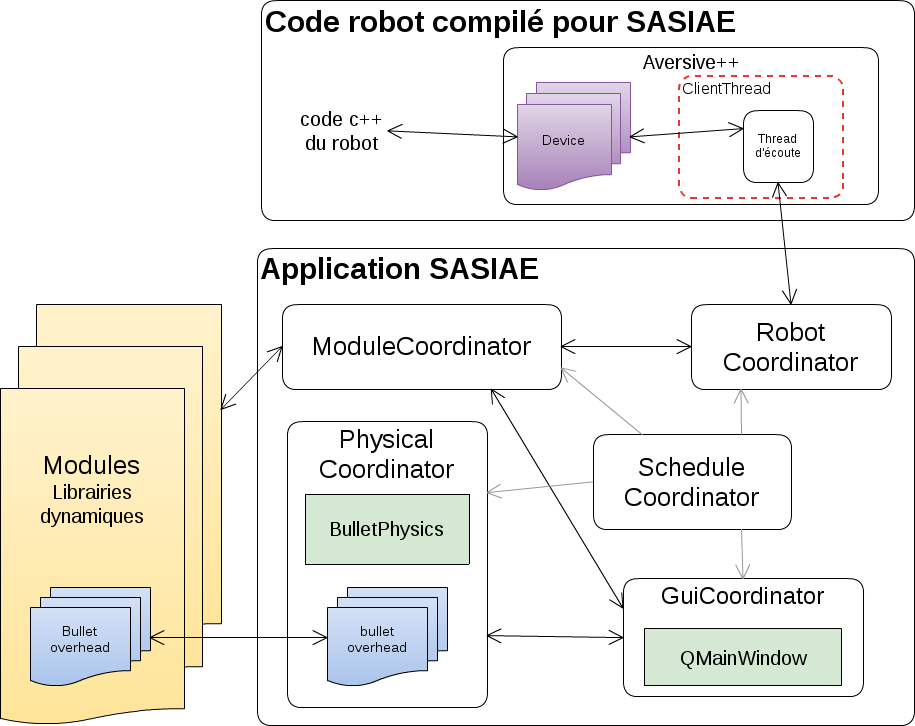
\includegraphics[width=\textwidth]{general}
\caption{Description générale du simulateur}
\label{descgenerale}
\end{figure}
\vspace{0 mm}
%\clearpage
L'architecture globale du projet est restée fidèle à celle du cahier des charges. Mais les difficultés rencontrées nous ont obligé à l'affiner quelque peu, comme par exemple l'éclatement du Coordinateur en plusieurs coordinateurs. Le détail des améliorations apportées sera effectué dans la section \ref{detail} et la figure \ref{descgenerale} reprend le schéma du cahier des charges enrichi des améliorations.

\section{Choix effectués}

\subsection{Contraintes de départ}

\paragraph{}
Il était prévu que plusieurs entités interagissent entre elles. Par conséquent nous voulions les abstraire le plus possible pour assurer l'indépendance des parties, le tout basé sur les conventions prises dans le cahier des charges. Pour ce faire, de nombreuses contraintes sont apparues dans l'écriture des classes intermédiaires. Ces contraintes de modularité et d'indépendance nous ont aussi amené à faire des choix que nous n'avions pas prévus dans le cahier des charges, comme par exemple la création d'une API pour le moteur de simulation physique. Celle-ci nous permet d'abstraire la communication avec Bullet.

De nombreuses semaines ont été nécessaires au lancement du projet pour pouvoir décider d'une architecture la plus cohérente possible. La taille du projet a fait que malgré toutes les précautions prises, il a fallu à quelques reprises revoir les choix que nous avions effectués.



%Du côté d'Aversive++, qui est le framework utilisé directement par le code robot, il a fallu abstraire la communication avec le reste du simulateur puisque les prototypes des classes et des méthodes employées est commun au simulateur et au robot. Il n'est donc pas question de lier ces classes au framework de Qt. Afin que tout puisse continuer à communiquer efficacement, malgré toutes les abstractions faites, il a fallu mettre l'accent sur le groupe des coordinateurs où chacun est dédié à la communication et synchronisation d'une partie spécifique du simulateur. 

\subsection{Programmation événementielle}

Pour rendre notre travail agréable à utilisé, il semble évident de faire une interface graphique. L'un des plus puissant framework libre actuel pour les réaliser est Qt. Or, ce framework nécessite de maîtriser un nouveau mode de programmation, la programmation événementielle. C'est un paradigme de programmation, à l'instar de la programmation séquentielle. Mais contrairement à cette dernière, au lieu de définir une séquence d'ordres donnés à la machine, la programmation événementielle consiste à définir comment l'application doit réagir lorsque tel ou tel événement se produit. Les événements auxquels peut réagir l'application sont nombreux et variés, allant de l'appui d'une touche au clavier, de la validation d'un formulaire ou d'un clic sur un bouton à un plus haut niveau mais aussi à l'arrivée d'un message réseau voire même l'envoi d'un message d'une entité interne à l'application. C'est dû à ce dernier point que la programmation événementielle est très souvent couplée avec l'orienté objet. En effet, les objets de l'application peuvent donc ainsi émettre des messages et d'autres objets qui écoutent ces messages réagiront en conséquence. De plus, la programmation événementielle permet une certaine aisance, facilitant la programmation d'interface graphique. En effet, pour la création d'interface graphique haut niveau, avec les outils adaptés, il suffit de placer les contrôles graphique de notre interface (menu déroulant, bouton, sélectionneur de couleur, etc) puis de définir le comportement de chacun des contrôles lorsqu'un événement utilisateur les concerne. Apprendre les mécanismes de cette méthode de programmation n'as pas été évident mais ce fut un réel enrichissement de notre culture technique. 


\section{Terminologie}
Nous allons aborder ici les quelques conventions utilisées par la suite. Tout d'abord, le projet comporte deux parties majeures qui sont l'API Aversive++ et le simulateur SASIAE, or ces deux entités possèdent théoriquement des implémentations de modules qui sont respectivement l'implémentation du code permettant d'exploiter un module et l'implémentation de l'image des actionneurs et des capteurs du Robot dans le simulateur. Les premiers seront donc nommés "device" par la suite tandis que les autres conservent le titre de "modules". De même, comme notre projet porte sur le monde de la robotique, le terme moteur physique portait à confusion. Nous appellerons donc calculateur physique les moteurs de calcul de la physique d'un environnement. Enfin, le projet nécessitait la mise en place d'un planificateur de tâches pour Aversive++ que nous avons nommé "Scheduler".




